\documentclass[a4paper,11pt]{article} %Selecionando a classe que gera artigos.

%PACOTES ABNT
\usepackage[brazil]{babel} % Pacote para usar portugues.
%Babel traduz como “table of contents“, “chapter” e “section“, sejam impressas como “sumário”, “capítulo” e “seção”, respectivamente.

\usepackage[T1]{fontenc} %Pacote para copiar palavras com acentuação do pdf de um documento feito em LaTeX que tenha usado esses pacotes resultará nas palavras corretamente acentuadas

\usepackage[utf8]{inputenc} % Pacote para poder usar acentuação no arquivo .tex

%\usepackage{biblatex}


\usepackage{graphicx} %Pacote para inserir Figuras.

\usepackage[top=2.0cm,right=2.0cm,left=2.0cm,bottom=2.0cm]{geometry} %Pacote de Margens

\usepackage{enumerate} %Pacote para usar marcadores.

\usepackage[onehalfspacing]{setspace} %Pacote espaçamento 1,5 cm.

\usepackage[alf]{abntex2cite} % configura o sistema  de citações e referências para o estilo ABNT.


% alf = estilo autor-data, para citações.

%Para mais estilos de citações visite https://www.overleaf.com/learn/latex/Biblatex_bibliography_styles

%PACOTES ESSENCIAIS
\usepackage{graphicx,xcolor,comment,enumerate,multirow,multicol,indentfirst} %Pacote para inserir figuras, tabelas, editar cores das tabelas, numeração "Automática das figuras e tabelas", identar tabelas e figuras.


%PACOTES DE MATEMÁTICA
\usepackage{amsmath,amsthm,amsfonts,amssymb,dsfont,mathtools,blindtext} %Pacotes básicos de matemática.

\usepackage{sectsty}% http://ctan.org/pkg/sectsty
\usepackage{titlecaps}% http://ctan.org/pkg/titlecaps
\sectionfont{\normalsize\MakeUppercase}


\usepackage{fancyhdr}  % Para adicionar o rodapé
 %Pacotes principais

\fancypagestyle{empty}{%
\fancyhf{}% clear all header and footer fields
\fancyfoot[L]{Linguagem e Descrição de Hardware} % except the center
\fancyfoot[R]{\thepage} % except the center
% \fancyfoot[R]{ISSN: 2178-9959} % except the center
\renewcommand{\headrulewidth}{0pt}%
\renewcommand{\footrulewidth}{0pt}%
}
\pagestyle{empty}

\begin{document} %Begin Inicia o Documento

%--------------------------------     NÃO ALTERAR    ----------------------------------------%
\begin{center}

% \begin{table}[!h]
% \centering
% \resizebox{\textwidth}{!}{
% \begin{tabular}{lr}
% %\multirow{4}{*}{
\includegraphics[width=80px]{logo_reitoria.png}} &
% % \multirow{6}{*}{
\includegraphics[width=120px]{logo_conict.png}}                                                                     & 
% % \multirow{6}{*}{
\includegraphics[width=190px]{logo_reitoria.png}} \\
% \multirow{1}{*}{
%   \centering
%   % 
\includegraphics[width=120px]{logo_conict.png}
%   } &
% \multirow{6}{*}{
%   \centering
%   
\includegraphics[width=130px]{logo_ifsp.png}
%   } \\
%                         &                                                        %                    &            
%                         \\
%                         &                                                         %                                    &                         
%                         \\
%                         & \multicolumn{1}{l}{\textbf{}}                          %                                     &                        
%                         \\
%                         & \multicolumn{1}{l}{\textbf{}}                          %                                     &                        
%                         \\
%                         %& 
%                         \multicolumn{2}{c}{\large{\textbf{Linguagem e Descrição de Hardware}}} \\
%                         %& \multicolumn{1}{l}{}   
% \end{tabular}
% }

% \end{table}

\begin{table}[!h]
  \centering
  \resizebox{\textwidth}{!}{
  \begin{tabular}{c}
  
\includegraphics[width=130px]{logo_ifsp.png} \\
  \large{\textbf{Linguagem e Descrição de Hardware}} \\
  \end{tabular}
  }
\end{table}

%-------------------------------------------------------------------------------------------------%



%%%%%%%%%%%%%%%%%%%%%%%%%%%%%  ALTERAR TÍTULO, AUTORES  %%%%%%%%%%%%%%%%%%%%%%%%%%%%%%%%%%%%%%%%%%%%%

\textbf{Greatest Common Divisor - (GCD)}\vspace{0.5cm}

Giovanna Fantacini$^1$, 
Higor Grigorio$^2$, 
Leonardo Reneres$^3$, 
Luis$^4$, 
Raul Prado Dantas$^5$


%%%%%%%%%%%%%%%%%%%%%%%%%%%%%%%%%%%%%%%%%%%%%%%%%%%%%%%%%%%%%%%%%%%%%%%%%%%%%%%%%%%%%%%%%%%%%%%%%%%%%





%----------------------------------APAGAR TABELA COMEÇO--------------------------------------------%

% \begin{table}[!h]
% \centering
% \resizebox{\textwidth}{!}{%
% \begin{tabular}{|c|}
% \hline
% {\color[HTML]{FE0000} \textbf{\begin{tabular}[c]{@{}c@{}}Não informe o nome dos autores na etapa de avaliação, apenas na versão final. \\
% O resumo expandido deve ter no máximo 6 (seis) páginas, incluindo as referências. \\
% O arquivo de submissão deve estar em formato .PDF.\\
% Remova este quadro antes do envio.\end{tabular}}} \\ \hline
% \end{tabular}%
% }
% \end{table}

%---------------------------------APAGAR TABELA FIM--------------------------------------------%


\end{center}

%%%%%%%%%%%%%%%%%%%%%%%%%%%%INSERIR INFORMAÇÕES ALUNOS%%%%%%%%%%%%%%%%%%%%%%%%%%%%%%%%%%%%%%%%%
% \begingroup
%     \fontsize{9pt}{11pt}\selectfont
  
%   $^1$Graduando em Tecnologia de Análise e Desenvolvimento de Sistemas, Bolsista PIBIFSP, IFSP, Câmpus Capivari, emailautor@ifsp.edu.br. (Times New Roman, 9, Justificado)
  
%   $^2$
  
%   $^3$
  
%   $^n$

% Área de conhecimento (Tabela CNPq): 1.03.03.04-9 Sistemas de Informação. 
% \endgroup

%%%%%%%%%%%%%%%%%%%%%%%%%%%%%%%%%%%%%%%%%%%%%%%%%%%%%%%%%%%%%%%%%%%%%%%%%%%%%%%%%%%%%%%%%%%%%%%% %Alterar Título, autores, e apagar tabela !

\begin{center}
    \tableofcontents %Gera o sumário
\end{center}

\newpage

%----------------------------------------TEXTOS-------------------------------------------------%

\vspace{0.5cm}
\noindent\textbf{RESUMO}: 
Este artigo apresenta a implementação do algoritmo para cálculo do 
Greatest Common Divisor (GCD) em hardware, 
utilizando uma abordagem de Control e Datapath. 
Serão abordadas as principais etapas de desenvolvimento, 
incluindo a descrição do algoritmo em linguagem C, 
a modelagem dos módulos de controle e datapath em Verilog, 
e a simulação e validação do sistema.

\vspace{0.5cm}
\noindent\textbf{PALAVRAS-CHAVE}: 
GCD; Greatest Common Divisor; Hardware Description Language; Control; Datapath;

\vspace{0.5cm}
 \begin{center}
 \textbf{Greatest Common Divisor - (GCD)}
 \end{center}

\noindent\textbf{ABSTRACT}: 
This paper presents the implementation of the Greatest Common Divisor (GCD) 
algorithm in hardware, using a Control and Datapath approach. 
The main development steps will be addressed, 
including the description of the algorithm in C language, 
the modeling of control and datapath modules in Verilog, 
and the system simulation and validation.

\vspace{0.5cm}
\noindent\textbf{KEYWORDS}: 
GCD; Greatest Common Divisor; Hardware Description Language; Control; Datapath;

\section{Introdução}

O Greatest Common Divisor (GCD) é um problema clássico da teoria dos números, 
com aplicações em diversas áreas da computação. 
Este trabalho baseia-se nas notas de aula da disciplina CSE 141L: 
Introduction to Computer Architecture Lab, 
ministrada na Universidade da Califórnia. 
O objetivo é desenvolver uma implementação eficiente do GCD 
utilizando linguagem de descrição de hardware.

O cálculo do GCD é frequentemente utilizado em algoritmos de criptografia, 
compressão de dados e outros campos onde operações matemáticas eficientes 
são essenciais. 
Este projeto visa criar um design em hardware que maximize a 
eficiência dessas operações.

As referências devem estar citadas no trabalho conforme a sua forma de citação, 
como por exemplo \cite{alves}, \cite{galvani} e \cite{national_instruments} 
ou em Pandorfi, et al, (2007). 
Na seção Referências devem ser listadas em ordem alfabética \cite{pandorfi}.

\section{Fundamentação Teórica} 
% Esta seção deve apresentar os conceitos teóricos fundamentais para o entendimento do GCD e sua relevância em computação. Aborde os princípios matemáticos e as aplicações típicas do GCD.

\subsection{Conceitos Básicos de GCD}
O conceito de Greatest Common Divisor (GCD), ou Máximo Divisor Comum (MDC) em português, é fundamental na teoria dos números e tem ampla aplicação em diversas áreas da matemática e da ciência da computação. O GCD de dois números inteiros é o maior número inteiro que divide ambos sem deixar resto. Esse conceito é importante não apenas na simplificação de frações, onde o GCD é utilizado para reduzir frações ao seu menor termo, mas também em áreas mais avançadas, como criptografia, teoria de algoritmos e circuitos digitais.

Na criptografia, por exemplo, o GCD desempenha um papel crítico em algoritmos de chave pública, como o RSA, onde o conceito de coprimosidade (números cujo GCD é 1) é utilizado para garantir a segurança do sistema. Em algoritmos, o GCD é frequentemente utilizado para otimizar cálculos que envolvem divisões e reduções, sendo a base de algoritmos clássicos como o Algoritmo de Euclides, que é amplamente utilizado por sua eficiência na computação do GCD.

No contexto de circuitos digitais, especificamente em módulos de controle e datapath, como os discutidos nos materiais analisados, o GCD pode ser implementado de forma eficiente através de circuitos que utilizam registradores, multiplexadores e unidades aritméticas. Esses componentes são coordenados por um módulo de controle que decide a sequência de operações, como subtrações e trocas de valores, até que o GCD seja obtido. A implementação eficiente desses circuitos é crucial para o desempenho de sistemas que exigem cálculos frequentes de GCD, especialmente em aplicações embarcadas e de tempo real.

Em resumo, o GCD não é apenas um conceito básico da matemática, mas também um elemento essencial em várias aplicações práticas, desde a simplificação de frações até sistemas complexos de criptografia e arquiteturas de hardware digital

\subsection{Algoritmo de Euclides}
O Algoritmo de Euclides é um dos métodos mais antigos e eficientes para calcular o Greatest Common Divisor (GCD), ou Máximo Divisor Comum (MDC), de dois números inteiros. Esse algoritmo, atribuído ao matemático grego Euclides, tem uma fundamentação simples e robusta, baseada na observação de que o GCD de dois números não muda se o maior dos dois números é substituído pela diferença entre eles. Essa propriedade permite a construção de um algoritmo iterativo que reduz progressivamente o problema até que o divisor comum seja encontrado.

O Algoritmo de Euclides funciona através de uma série de divisões sucessivas. Dado dois números inteiros \( A \) e \( B \), onde \( A \geq B \), o algoritmo segue os seguintes passos:

\begin{enumerate}
    \item \textbf{Divisão}: Divida \( A \) por \( B \) e obtenha o quociente \( q \) e o resto \( r \) tal que \( A = Bq + r \).
    \item \textbf{Substituição}: Substitua \( A \) por \( B \) e \( B \) por \( r \).
    \item \textbf{Repetição}: Repita os passos acima até que \( r \) seja igual a zero. Quando isso acontecer, o GCD é o valor de \( B \) naquele ponto.
\end{enumerate}

Matematicamente, isso pode ser representado como:

\[
\text{GCD}(A, B) = \text{GCD}(B, A \mod B)
\]

Quando \( B \) se torna zero, \( A \) contém o GCD dos dois números iniciais.

Considere a aplicação do algoritmo para encontrar o GCD de 48 e 18:

\begin{itemize}
    \item \( 48 \div 18 = 2 \) com resto 12 (\( 48 = 18 \times 2 + 12 \)).
    \item Substitua \( A = 18 \) e \( B = 12 \).
    \item \( 18 \div 12 = 1 \) com resto 6 (\( 18 = 12 \times 1 + 6 \)).
    \item Substitua \( A = 12 \) e \( B = 6 \).
    \item \( 12 \div 6 = 2 \) com resto 0 (\( 12 = 6 \times 2 + 0 \)).
\end{itemize}

Como o resto é zero, o GCD é 6.

O Algoritmo de Euclides é conhecido por sua eficiência. A cada iteração, o tamanho dos números envolvidos é reduzido, e em média, o número de iterações necessárias é proporcional ao logaritmo do menor número entre os dois. A complexidade computacional do algoritmo é \( O(\log(\min(A, B))) \), o que o torna extremamente eficiente mesmo para números muito grandes.

A eficiência do Algoritmo de Euclides o torna preferido em muitos contextos de aplicação, desde cálculos aritméticos básicos até implementações em hardware e criptografia, onde cálculos rápidos e precisos do GCD são frequentemente necessários.

\subsection{Aplicações do GCD em Computação}
O \textit{Greatest Common Divisor} (GCD), ou Máximo Divisor Comum (MDC), é uma operação fundamental com diversas aplicações práticas em computação. Sua relevância se estende desde algoritmos básicos até sistemas complexos de criptografia, compressão de dados e implementação em hardware.

Uma das aplicações mais notáveis do GCD está na criptografia, especialmente em sistemas de criptografia assimétrica, como o algoritmo RSA. O RSA depende da dificuldade de fatorar grandes números primos, e a função GCD é usada para determinar se dois números são \textit{coprimos}, ou seja, se seu GCD é 1. A coprimosidade é um conceito crucial no processo de geração de chaves no RSA, onde o GCD garante que a chave pública e o módulo sejam adequados para a operação de criptografia e descriptografia.

Outra aplicação importante do GCD é na compressão de dados. Técnicas de compressão como o \textit{Run-Length Encoding} (RLE) podem utilizar o GCD para determinar padrões de repetição e reduzir a redundância nos dados. Além disso, algoritmos de compressão baseados em análise de fatores de números, como o \textit{factoring-based compression}, usam o GCD para simplificar expressões numéricas e otimizar o armazenamento.

Em \textbf{sistemas de controle}, especialmente em hardware, o GCD é utilizado para simplificar os cálculos que envolvem múltiplos ciclos de operação ou para sincronizar sinais em circuitos digitais. No contexto de \textit{Control and Datapath}, a operação de GCD pode ser implementada em circuitos que exigem operações de redução, como divisões sucessivas, facilitando a minimização de recursos computacionais.

A operação de GCD é relevante em hardware porque ela pode ser implementada de forma eficiente utilizando componentes básicos como registradores, multiplexadores e subtratores, que são comuns em \textit{datapaths} de circuitos digitais. A eficiência do GCD, especialmente quando implementado com o \textit{Algoritmo de Euclides}, permite que ele seja utilizado em sistemas de tempo real e em dispositivos embarcados, onde a velocidade de processamento e o uso mínimo de recursos são críticos. Além disso, o GCD é frequentemente empregado em \textbf{algoritmos de síntese lógica} para otimizar o design de circuitos e na verificação formal de \textit{hardware}.

Em resumo, o GCD é uma operação essencial em diversas áreas da computação, proporcionando uma base sólida para algoritmos criptográficos, técnicas de compressão de dados e a implementação eficiente de sistemas de controle em \textit{hardware} digital.


\section{Desenho de Arquitetura}
% Nesta seção, descreva a arquitetura utilizada para a implementação do GCD em hardware. 
% Inclua uma visão geral dos módulos e suas interações.
Esta seção descreve a arquitetura do sistema, 
incluindo a partição em módulos de controle e datapath, 
e os diagramas de blocos que ilustram a interação entre os componentes.

\subsection{Partição em Módulos}
% Detalhamento da divisão do projeto em módulos de Control e Datapath. 
% Explicar o papel de cada módulo no sistema e como eles se comunicam. 
% Pode incluir um diagrama de blocos para ilustrar.
A arquitetura do sistema GCD foi organizada em dois módulos principais: Control e Datapath.
Esta divisão permite uma clara separação de responsabilidades, permite 
uma maior modularidade, 
facilita a implementação, manutenção e expansão do sistema.

\subsubsection{Módulo de Controle}
O módulo de Controle é responsável por gerenciar o fluxo de dados 
entre os diferentes componentes do sistema e controlar as transições de estado. 
Ele coordena as operações do Datapath com base nas condições de controle, 
assegurando que as etapas do cálculo do GCD sejam executadas na ordem correta. 
Este módulo inclui uma Máquina de Estados Finitos (FSM), a qual será discutida posteriormente,
que determina a sequência de operações, incluindo a inicialização, 
execução do cálculo e término.

\subsubsection{Módulo Datapath}
O Datapath realiza as operações aritméticas necessárias para o cálculo do GCD, 
como subtrações e comparações entre os valores de entrada. 
Este módulo contém registradores, multiplexadores, e a unidade de subtração, 
que juntos formam o núcleo da operação matemática. 
A eficiência do Datapath é crítica para o desempenho global do sistema, 
uma vez que ele executa as operações fundamentais repetidamente até 
que o resultado seja obtido.


\subsection{Diagramas de Blocos}
% Apresentar diagramas de blocos que representem a arquitetura do GCD, 
% mostrando como os diferentes componentes se conectam e interagem. 
% Explicar o fluxo de dados entre os módulos.
O diagrama de bloco na Figura \ref{fig:top_level} 
ilustra a arquitetura de nível superior do sistema GCD, 
apresentando todas as entradas e saídas em um único bloco. 
Este diagrama de blocos demonstra como os módulos de 
Controle e Datapath estão interconectados e como o fluxo de dados é gerenciado entre eles. 

\begin{figure}[ht]
    \centering
    \caption{Diagrama de Blocos do Sistema GCD}
    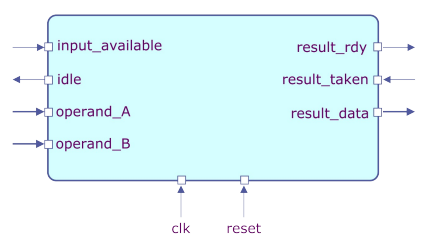
\includegraphics[width=15cm,angle=0]{imgs/diagram_block_top_level.png}
    \\\textbf{Fonte:} \cite{cse_taylor_michael}
    \label{fig:top_level}
\end{figure}

O diagrama de blocos na Figura \ref{fig:diagram_block} ilustra como os componentes principais 
do sistema GCD se interconectam. 

\begin{figure}[ht]
    \centering
    \caption{Diagrama de Blocos do Sistema GCD}
    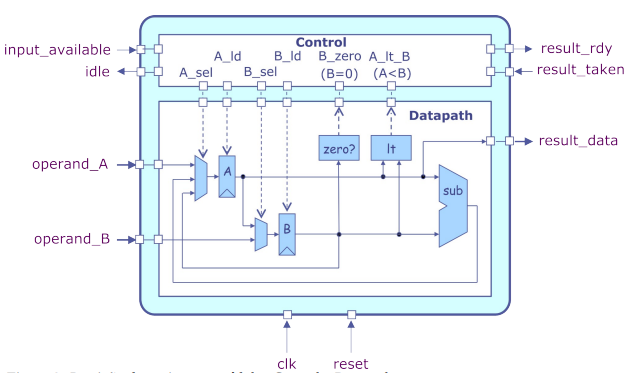
\includegraphics[width=17cm,angle=0]{imgs/diagram_block_control_datapath.png}
    \\\textbf{Fonte:} \cite{cse_taylor_michael}
    \label{fig:diagram_block}
\end{figure}

O Datapath inclui os registradores, multiplexadores e a unidade de subtração, 
enquanto o Control FSM gerencia as operações com base nos sinais de controle.

\clearpage
\section{Desenvolvimento e Implementação}

Os materiais e métodos utilizados no desenvolvimento da pesquisa 
incluem a descrição do algoritmo em C e
a modelagem dos módulos de controle e datapath em Verilog.
Além da simulação utilizando o ambiente Intel Quartus.

\subsection{Descrição do Algoritmo em C}

O código a seguir é uma implementação da função GCD (Greatest Common Divisor - Maior Divisor Comum). 
Essa função calcula o maior divisor comum entre dois números inteiros.

A função GCD recebe dois parâmetros: inA e inB, 
que representam os dois números inteiros para os quais 
queremos calcular o maior divisor comum.

O código utiliza um algoritmo chamado "algoritmo de Euclides" 
para calcular o maior divisor comum. 
O algoritmo de Euclides é baseado na observação de que 
o maior divisor comum entre dois números não muda 
se o menor número for subtraído do maior número repetidamente 
até que um dos números seja igual a zero.

O algoritmo para cálculo do GCD pode ser implementado de diversas maneiras. 
Abaixo, apresentamos uma implementação em linguagem C:

\begin{verbatim}
int GCD(int inA, int inB) {
    int swap;
    int done = 0;
    int A = inA;
    int B = inB;
    while (!done) {
        if (A < B) {
            swap = A;
            A = B;
            B = swap;
        } else if (B != 0) {
            A = A - B;
        } else {
            done = 1;
        }
    }
    return A;
}
\end{verbatim}


Aqui está uma explicação passo a passo do funcionamento do código:

\begin{enumerate}
    \item O código declara algumas variáveis locais: \begin{verbatim}swap\end{verbatim}, \begin{verbatim}done\end{verbatim}, \begin{verbatim}A\end{verbatim} e \begin{verbatim}B\end{verbatim}.
    \begin{verbatim}swap\end{verbatim} é usada para trocar os valores de \begin{verbatim}A\end{verbatim} e \begin{verbatim}B\end{verbatim} quando necessário.
    \begin{verbatim}done\end{verbatim} é uma variável de controle que indica se o cálculo do maior divisor comum está concluído.
    \begin{verbatim}A\end{verbatim} e \begin{verbatim}B\end{verbatim} são inicializadas com os valores dos parâmetros \begin{verbatim}inA\end{verbatim} e \begin{verbatim}inB\end{verbatim}, respectivamente.
    \item O código entra em um loop \begin{verbatim}while\end{verbatim} que continua até que a variável \begin{verbatim}done\end{verbatim} seja igual a 1.
    \item O loop é usado para realizar as iterações necessárias para calcular o maior divisor comum.
    \item Dentro do loop, há uma estrutura \begin{verbatim}if-else\end{verbatim} que verifica três condições:
    \begin{enumerate}
        \item Se \begin{verbatim}A\end{verbatim} for menor que \begin{verbatim}B\end{verbatim}, os valores de \begin{verbatim}A\end{verbatim} e \begin{verbatim}B\end{verbatim} são trocados usando a variável \begin{verbatim}swap\end{verbatim}. Isso garante que \begin{verbatim}A\end{verbatim} seja sempre o maior número.
        \item Se \begin{verbatim}B\end{verbatim} for diferente de zero, \begin{verbatim}A\end{verbatim} é atualizado para \begin{verbatim}A - B\end{verbatim}. Isso realiza a subtração repetida até que um dos números seja igual a zero.
        \item Se nenhuma das condições anteriores for verdadeira, significa que o cálculo do maior divisor comum está concluído e a variável \begin{verbatim}done\end{verbatim} é definida como 1 para sair do loop.
    \end{enumerate}
    \item Após o loop, o código retorna o valor de \begin{verbatim}A\end{verbatim}, que representa o maior divisor comum entre os números \begin{verbatim}inA\end{verbatim} e \begin{verbatim}inB\end{verbatim}.
\end{enumerate}

Por exemplo, se chamarmos a função GCD(24, 36), o algoritmo de Euclides será aplicado da seguinte maneira:

\begin{enumerate}
    \item Na primeira iteração, \begin{verbatim}A\end{verbatim} é atualizado para 36 e \begin{verbatim}B\end{verbatim} é atualizado para 24.
    \item Na segunda iteração, \begin{verbatim}A\end{verbatim} é atualizado para 12 e \begin{verbatim}B\end{verbatim} é atualizado para 24.
    \item Na terceira iteração, \begin{verbatim}A\end{verbatim} é atualizado para 12 e \begin{verbatim}B\end{verbatim} é atualizado para 12.
    \item Na quarta iteração, \begin{verbatim}A\end{verbatim} é atualizado para 0 e \begin{verbatim}B\end{verbatim} é atualizado para 12.
    \item Como \begin{verbatim}B\end{verbatim} é igual a zero, o cálculo do maior divisor comum está concluído e o valor retornado é 12.
\end{enumerate}


\subsection{Modelagem em Verilog}

A implementação do GCD em hardware envolve a 
criação de módulos para o controle e o datapath. 
O datapath lida com a movimentação e transformação dos dados, 
enquanto o módulo de controle gerencia as operações de controle.

\subsubsection{Módulo Datapath}

O código a seguir é um exemplo de um módulo em Verilog 
que implementa o datapath para um algoritmo de cálculo do 
Máximo Divisor Comum (GCD - Greatest Common Divisor). 

\begin{verbatim}
module GCDdatapath#( parameter W=16 )
(
    input clk,
    input [W-1:0] operand_A,
    input [W-1:0] operand_B,
    output [W-1:0] result_data,
    input A_ld,
    input B_ld,
    input [1:0] A_sel,
    input B_sel,
    output B_zero,
    output A_lt_B,
    output [W-1:0] A_chk, B_chk, sub_chk, A_mux_chk, B_mux_chk
);

    wire [W-1:0] A;
    wire [W-1:0] B;
    wire [W-1:0] sub_out;
    wire [W-1:0] A_mux_out;
    wire [W-1:0] B_mux_out;

    Mux3#(W) A_mux(
        .in0 (operand_A),
        .in1 (sub_out),
        .in2 (B),
        .sel (A_sel),
        .out (A_mux_out) 
    );

    register#(W) A_reg (
        .clk (clk),
        .d (A_mux_out),
        .en (A_ld),
        .q (A) 
    );

    Mux2#(W) B_mux (
        .in0 (A),
        .in1 (operand_B),
        .sel (B_sel),
        .out (B_mux_out) 
    );

    register#(W) B_reg (
        .clk (clk),
        .d (B_mux_out),
        .en (B_ld),
        .q (B) 
    );

    assign B_zero = (B==0);
    assign A_lt_B = (A < B);
    assign sub_out = A - B;
    assign result_data = A;
    // send checking signals only for debugging purposes
    assign A_chk = A;
    assign B_chk = B;
    assign sub_chk = sub_out;
    assign A_mux_chk = A_mux_out;
    assign B_mux_chk = B_mux_out;
endmodule
\end{verbatim}


A seguir, o funcionamento do código passo a passo:

O módulo GCDdatapath recebe alguns parâmetros, 
sendo o principal deles W, 
que define o tamanho dos operandos e do resultado em bits.

O módulo possui várias entradas e saídas, incluindo:

\begin{itemize}
    \item \begin{verbatim}clk\end{verbatim}: um sinal de clock para sincronizar as operações.
    \item \begin{verbatim}operand_A\end{verbatim} e \begin{verbatim}operand_B\end{verbatim}: os operandos de entrada para o cálculo do GCD.
    \item \begin{verbatim}result_data\end{verbatim}: o resultado do cálculo do GCD.
    \item \begin{verbatim}A_ld\end{verbatim} e \begin{verbatim}B_ld\end{verbatim}: sinais de controle para carregar os operandos A e B.
    \item \begin{verbatim}A_sel\end{verbatim} e \begin{verbatim}B_sel\end{verbatim}: sinais de seleção para escolher entre os operandos A e B.
    \item \begin{verbatim}B_zero\end{verbatim}: um sinal indicando se o operando B é igual a zero.
    \item \begin{verbatim}A_lt_B\end{verbatim}: um sinal indicando se o operando A é menor que o operando B.
    \item \begin{verbatim}A_chk\end{verbatim}, \begin{verbatim}B_chk\end{verbatim}, \begin{verbatim}sub_chk\end{verbatim}, \begin{verbatim}A_mux_chk\end{verbatim} e \begin{verbatim}B_mux_chk\end{verbatim}: sinais de depuração para verificar os valores internos do datapath.
\end{itemize}


O módulo possui várias fiações (wires) para conectar os componentes internos:

\begin{verbatim}A, B, sub_out, A_mux_out\end{verbatim} e \begin{verbatim}B_mux_out\end{verbatim}: fiações para transportar os valores dos operandos e resultados intermediários.

O módulo utiliza vários componentes internos para realizar as operações do datapath:

\begin{itemize}
    \item \begin{verbatim}Mux3#(W) A_mux\end{verbatim}: um multiplexador de 3 entradas que seleciona entre o operando A, o resultado da subtração e o operando B, com base no sinal de seleção \begin{verbatim}A_sel\end{verbatim}. O resultado é armazenado em \begin{verbatim}A_mux_out\end{verbatim}.
    \item \begin{verbatim}register#(W) A_reg\end{verbatim}: um registrador que armazena o valor de \begin{verbatim}A_mux_out\end{verbatim} e o atualiza no sinal de clock \begin{verbatim}clk\end{verbatim} quando o sinal de controle \begin{verbatim}A_ld\end{verbatim} está ativo. O valor atualizado é armazenado em \begin{verbatim}A\end{verbatim}.
    \item \begin{verbatim}Mux2#(W) B_mux\end{verbatim}: um multiplexador de 2 entradas que seleciona entre o valor atualizado de \begin{verbatim}A\end{verbatim} e o operando \begin{verbatim}B\end{verbatim}, com base no sinal de seleção \begin{verbatim}B_sel\end{verbatim}. O resultado é armazenado em \begin{verbatim}B_mux_out\end{verbatim}.
    \item \begin{verbatim}register#(W) B_reg\end{verbatim}: um registrador que armazena o valor de \begin{verbatim}B_mux_out\end{verbatim} e o atualiza no sinal de clock \begin{verbatim}clk\end{verbatim} quando o sinal de controle \begin{verbatim}B_ld\end{verbatim} está ativo. O valor atualizado é armazenado em \begin{verbatim}B\end{verbatim}.
\end{itemize}

As atribuições assign são usadas para definir os valores das saídas do módulo:

\begin{itemize}
    \item \begin{verbatim}B_zero\end{verbatim} é atribuído como verdadeiro se o valor de \begin{verbatim}B\end{verbatim} for igual a zero.
    \item \begin{verbatim}A_lt_B\end{verbatim} é atribuído como verdadeiro se o valor de \begin{verbatim}A\end{verbatim} for menor que o valor de \begin{verbatim}B\end{verbatim}.
    \item \begin{verbatim}sub_out\end{verbatim} é atribuído como a diferença entre \begin{verbatim}A\end{verbatim} e \begin{verbatim}B\end{verbatim}.
    \item \begin{verbatim}result_data\end{verbatim} é atribuído como o valor de \begin{verbatim}A\end{verbatim}.
    \item Os sinais de depuração \begin{verbatim}A_chk\end{verbatim}, \begin{verbatim}B_chk\end{verbatim}, \begin{verbatim}sub_chk\end{verbatim}, \begin{verbatim}A_mux_chk\end{verbatim} e \begin{verbatim}B_mux_chk\end{verbatim} são atribuídos aos respectivos valores internos do datapath.
\end{itemize}

O módulo GCDdatapath encapsula todas essas operações e fiações para formar um datapath completo para o cálculo do GCD.


\subsubsection{Módulo Controle}
\begin{verbatim}
module GCDcontrol(
    input input_available,
    output reg idle,
    input clk, reset,
    output reg A_ld, B_sel, B_ld,
    output reg [1:0] A_sel,
    input B_zero, A_lt_B,
    output reg result_rdy,
    input result_taken,
    output [1:0] State
);

    // States naming
    localparam WAIT = 2'd0;
    localparam CALC = 2'd1;
    localparam DONE = 2'd2;

    // Constants naming for A_mux selector
    localparam A_SEL_IN = 2'b00;
    localparam A_SEL_SUB = 2'b01;
    localparam A_SEL_B = 2'b10;
    localparam A_SEL_X = 2'b11;
    // Constants naming for B_mux selector
    localparam B_SEL_A = 1'b0;
    localparam B_SEL_IN = 1'b1;
    localparam B_SEL_X = 1'bx;

    reg [1:0] CurrentState, NextState;

    always @(posedge clk or posedge reset)  
    begin 
        if (reset) 
            CurrentState <= WAIT;
        else 
            CurrentState <= NextState; 
    end 

    always @(CurrentState)
    begin
        // default is to stay in the same state
        NextState <= CurrentState;
        case ( CurrentState )
            WAIT :
                if ( input_available )
                    NextState <= CALC;
            CALC :
                if ( B_zero )
                    NextState <= DONE;
            DONE :
                if ( result_taken )
                    NextState <= WAIT;
        endcase
    end 

    always @( * )
    begin
        // Default control signals
        A_sel <= A_SEL_X;
        A_ld <= 1'b0;
        B_sel <= B_SEL_X;
        B_ld <= 1'b0;
        idle <= 1'b0; 
        result_rdy = 1'b0;

        case ( CurrentState )
            WAIT :
                begin
                    idle <= 1'b1; 
                    if(input_available)begin
                        A_sel <= A_SEL_IN;
                        B_sel <= B_SEL_IN;
                        A_ld <= 1'b1;   
                        B_ld <= 1'b1;
                    end
                end
            CALC :
                if ( A_lt_B )begin
                    A_sel <= A_SEL_B;
                    B_sel <= B_SEL_A;
                    A_ld <= 1'b1;
                    B_ld <= 1'b1;
                end
                else if ( !B_zero )begin
                    A_sel <= A_SEL_SUB;
                    A_ld <= 1'b1;
                end
            DONE : 
                result_rdy <= 1'b1;
        endcase
    end

    assign State = CurrentState;
endmodule
\end{verbatim}

\section{Máquina de Estados Finitos (FSM)}
% Nesta seção, discuta a FSM utilizada para controlar o Datapath.

\subsection{Descrição dos Estados}
% Descrever os diferentes estados da FSM, explicando o que ocorre em cada estado e como as transições entre estados são gerenciadas. Pode incluir um diagrama de estados para visualização.

\subsection{Implementação da FSM}
% Discutir como a FSM foi implementada em Verilog, incluindo os desafios encontrados durante o desenvolvimento e como foram superados. Explicar a lógica de transição e os sinais de controle envolvidos.

\section{Simulações e Verificação}

Para validar a implementação, foi realizada a simulação dos módulos utilizando o ambiente Intel QuestaSim. A Figura \ref{fig:simulacao} mostra a simulação do módulo GCD.

\subsection{Simulação do módulo GCD}
\begin{figure}[ht]
\centering
% \includegraphics[width=10cm,angle=0]{simulacao_gcd.png}
\caption{Simulação do módulo GCD}
\label{fig:simulacao}
\end{figure}

Os resultados da simulação confirmam que o design do GCD em hardware funciona conforme esperado. O módulo datapath executa corretamente as operações de subtração e troca, enquanto o módulo de controle gerencia os estados do sistema de maneira eficiente.

\subsection{Ambiente de Simulação}
% Descrever o ambiente de simulação utilizado, como o Intel QuestaSim. Explicar como os testes foram configurados e quais aspectos do sistema foram verificados.

\subsection{Resultados da Simulação}
% Apresentar os resultados obtidos durante a simulação. Incluir gráficos ou capturas de tela que mostrem a operação do GCD. Discutir se os resultados atenderam às expectativas e os objetivos do projeto.

\section{Otimizações e Melhorias Futuras}
% Discutir possíveis otimizações no design e propostas para futuras melhorias.

\subsection{Otimização do Datapath}
% Sugerir melhorias no Datapath, como a implementação de pipelining para aumentar a eficiência. Discutir possíveis modificações que poderiam ser feitas para melhorar o desempenho geral do sistema.

\subsection{Expansão do Design para Sistemas Maiores}
% Discutir como o design do GCD poderia ser expandido para se integrar com sistemas maiores ou suportar operações mais complexas. Propor ideias para a adaptação do módulo para novas aplicações.

\section{Discussão sobre Integração com Sistemas Maiores}
% Explorar como o módulo GCD poderia ser integrado em sistemas mais complexos, como processadores ou coprocessadores específicos para criptografia. Discutir os desafios de integração e as vantagens dessa abordagem.

\section{Conclusões}

Neste artigo, apresentamos a implementação do algoritmo GCD em hardware, detalhando a modelagem dos módulos de controle e datapath em Verilog. A simulação mostrou que a abordagem utilizada é eficiente e atende aos requisitos do projeto. Futuras melhorias podem incluir a otimização do datapath e a integração com outros módulos de um sistema maior.

%Referências Bibliográficas
\bibliography{bibliografia.bib}
%\printbibliography[title={REFERÊNCIAS}]
%\printbibliography{bibliografia}

\end{document}
